% Interpreting a case by comparing its results on two application versions.
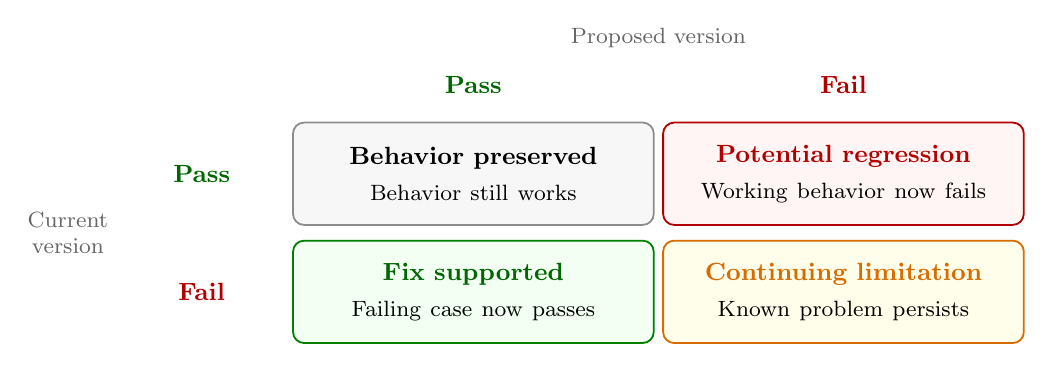
\begin{tikzpicture}[
  badge/.style={font=\small\bfseries, minimum height=0.5cm, inner sep=3pt},
  pass/.style={badge, text=green!40!black},
  fail/.style={badge, text=red!70!black},
  axis/.style={font=\footnotesize, text=black!60, align=center,
    inner sep=0pt},
  cell/.style={rounded corners=4pt, line width=0.65pt, align=center,
    minimum width=4.5cm, minimum height=1.3cm, text width=4.3cm,
    inner sep=4pt}
]
  % Column axis: result on the proposed version.
  \node[axis] at (8.3,0) {Proposed version};
  \node[pass] at (5.95,-0.6) {Pass};
  \node[fail] at (10.65,-0.6) {Fail};

  % Row axis: result on the previous version.
  \node[axis] at (0.8,-2.48) {Current\\version};
  \node[pass] at (2.5,-1.73) {Pass};
  \node[fail] at (2.5,-3.23) {Fail};

  % Interpretation of each combination.
  \node[cell, draw=black!45, fill=black!3] at (5.95,-1.73)
    {\small\textbf{Behavior preserved}\\[1pt]
     {\footnotesize Behavior still works}};
  \node[cell, draw=red!70!black, fill=red!4] at (10.65,-1.73)
    {\small\textbf{\textcolor{red!70!black}{Potential regression}}\\[1pt]
     {\footnotesize Working behavior now fails}};
  \node[cell, draw=green!50!black, fill=green!5] at (5.95,-3.23)
    {\small\textbf{\textcolor{green!40!black}{Fix supported}}\\[1pt]
     {\footnotesize Failing case now passes}};
  \node[cell, draw=orange!85!black, fill=yellow!8] at (10.65,-3.23)
    {\small\textbf{\textcolor{orange!85!black}{Continuing limitation}}\\[1pt]
     {\footnotesize Known problem persists}};
\end{tikzpicture}
